\documentclass[12pt]{spieman}  % 12pt font required by SPIE;
%\documentclass[a4paper,12pt]{spieman}  % use this instead for A4 paper
\usepackage{amsmath,amsfonts,amssymb}
\usepackage{graphicx}
\usepackage{setspace}
\usepackage{tocloft}

\title{Photometric \& Spectral Calibration of the Solar Ultraviolet Imaging Telescope on-board Aditya-L1}

\author[a]{First Author}
\author[a]{Second Author}
\author[b]{Third Author}
\author[a,b,*]{Fourth Author}
\affil[a]{University Name, Faculty Group, Department, Street Address, City, Country, Postal Code}
\affil[b]{Company Name, Street Address, City, Country, Postal Code}

%%%%%%%%%%%%% ############# %%%%%%%%%%%
\newcommand{\isro}{{\it ISRO}}
\newcommand{\suit}{{\it SUIT~}}
\newcommand{\degree}{$^{\circ}$}
\newcommand{\sr}[1]{{\bf\color{red} [#1]}}
\newcommand{\dt}[1]{{\bf\color{blue} [#1]}}
\newcommand{\js}[1]{{\bf\color{magenta} [#1]}}

%%%%%%%%%%%%% ############  %%%%%%%%%%%


\graphicspath{{./}{pics/}}
\renewcommand{\cftdotsep}{\cftnodots}
\cftpagenumbersoff{figure}
\cftpagenumbersoff{table} 
\begin{document} 
\maketitle

\begin{abstract}
The Solar Ultraviolet Imaging Telescope (\suit) is one of the 7 payloads on board the Aditya-L1 mission of the Indian Space Research Organization (\isro). \suit will provide full as well as partial disk images of the Sun in the wavelength range of 200{--}400 nm. This would help us probe the solar atmosphere at different heights and understand the process of mass and energy transfer between layers. \suit will also help us measure spatially resolved solar spectral irradiance at the wavelengths significant for the Sun-Climate relationship studies for the very first time. In this article, we present the methodology and results for photometric and spectral characterization of the payload across its 11 available science filter combinations.  
\end{abstract}

% Include a list of up to six keywords after the abstract
\keywords{optics, photonics, light, solar, NUV, sun-climate, irradiance}

% Include email contact information for corresponding author
{\noindent \footnotesize\textbf{*}Fourth author name,  \linkable{myemail@university.edu} }

%\begin{spacing}{2}   % use double spacing for rest of manuscript

%xxxxxxxxxxxxxxxxxxxxxxxxxxxxxxxxxxxxxxxxxxxxxxxxxxxxxxxxxxxxxxxxxxxxxxxxxxxxxxxxxxxxxxxxxxxxxxxxx
%%%%%%%%%%%%%%%%%%%%%%%%%%%%%%%%%%%%%%%%%%%%%%%%
\section{Introduction}\label{sec:intro}
%%%%%%%%%%%%%%%%%%%%%%%%%%%%%%%%%%%%%%%%%%%%%%%%

The Solar Ultraviolet Imaging Telescope(\suit) \cite{ghosh16,article} is an instrument on-board Aditya{--}L1 mission \cite{adityal1,aditya} of the Indian Space Research Organization (\isro) launched on September 2, 2023, that would measure the solar radiation in the near ultraviolet range (200{--}400 nm). \suit, with its 11 scientific bandpasses (3 broadband and 8 narrowband) will have the capability to probe different heights of solar atmosphere in the photosphere and the chromosphere. This will help us understand the different processes that transport mass and energy from one layer to another. \suit will provide full disk as well as partial disk images of the Sun with a plate scale of 0.7"/px.

 With \suit imaging we would be able to resolve solar flares spatially on the surface of the Sun, in near ultra-violet (NUV), which will help us to address the questions regarding their build-up and triggering mechanisms. In addition, \suit shall make spatially resolved solar spectral irradiance measurements within the wavelength range required to study the chemistry of oxygen and ozone in the Earth's stratosphere.

\suit has two main sub-units - the optical bench and the payload electronics. Atop the optical bench is an off-axis Ritchey Chreiten type telescope, specially designed to observe the sun in NUV.The main components constitute of a multi-operation entrance-door mechanism, thermal filter- to control the amount of incoming sunlight, primary and secondary mirrors, a shutter mechanism to control exposures, baffles to reduce scattering and stray light, a motorized filter wheel assembly, a piezoelectric focusing mechanism and a CCD detector. Fig \ref{fig:suit} shows a schematic diagram of the payload.

%------------------------------------------------------------
\begin{figure}[ht!]
\begin{center}
\begin{tabular}{c}
\includegraphics[width=0.8\linewidth]{SUITLayout.jpg}
\end{tabular}
\end{center}
\caption 
{ \label{fig:suit} A schematic diagram of \suit payload with various components as labeled. } 
\end{figure} 
%-----------------------------------------------------------

The \suit filter wheel assembly is responsible for selecting the desired filter combination among the 11 bandpasses to observe the requisite layer of the solar atmosphere. This is facilitated by a collection of 16 science filters, mounted on two 8-position filter wheels. The science filters are designed to balance the fluxes at the detector in different bands, to keep it within the dynamic range, while providing the needed bandpass. This is necessary as the Solar flux increases by almost a factor of 20 in the wavelength range of 200{--}400 nm, shown in Fig. \ref{fig:sun_spec} taken from \href{https://www.stsci.edu/hst/instrumentation/reference-data-for-calibration-and-tools/astronomical-catalogs/calspec}{CALSPEC} \cite{bohlin14,bohlin20,bohlin22} database. The two filter wheels can be rotated independently to achieve the desired filter combination within the beam path. Table \ref{tab:science_filters} gives the details of all 11 science bandpasses and the required filter combination for optimum throughput.

%-----------------------------------------------------------
\begin{table*}[ht]
\caption{List of science filters on board \suit. The columns from left to right denote: filter abbreviations, central wavelengths for science filters, corresponding bandpass, Nominal exposure time for a full disk observation the science target of the band.} 
\label{tab:science_filters}
\begin{center}
\begin{tabular}{||l|c|c|c|c|r||}
\hline
\textbf{Science}  &	\textbf{Combination} &	\textbf{Central} & \textbf{Bandpass}& \textbf{Nominal} &\textbf{Science} \\
\textbf{Filter}	&	\textbf{Filter}     &	\textbf{Wavelength  (nm)}	&		\textbf{(nm)	}	    & \textbf{Exp. Time (s)}	&\textbf{target}		\\
\hline
NB1     & BB1 		& 214.0 		    & 11.0 		&		& Continuum\\
NB2 	& BP2		& 276.7				& 0.4 		&		& Mg~\rm{II}~k blue wing \\
NB3 	& BP2		& 279.6 			& 0.4 		&		& Mg~\rm{II}~k\\
NB4 	& BP2		& 280.3				& 0.4 		&		& Mg~\rm{II}~h\\
NB5		& BP2		& 283.2				& 0.4 		&		& Mg~\rm{II}~h red wing\\
NB6 	& BP3		& 300.0 			&1.0 		&		& Continuum\\
NB7 	& BP3		& 388.0				&1.0 		&		& Continuum\\
NB8		& NB8		& 396.85 			& 0.1 		&		& Ca~\rm{II}~h\\
BB1 	& BB1		& 220.0				& 40.0 		&		& Herzberg Continuum \\
BB2 	& BP4		& 277.0 			& 58.0       &       & Hartley Band\\
BB3 	& BP4		& 340.0				& 40.0        &      & Huggins Band\\
\hline
\end{tabular}
\end{center}
\end{table*}
%-----------------------------------------------------------

%------------------------------------------------------------
\begin{figure}[ht]
\begin{center}
\begin{tabular}{c}
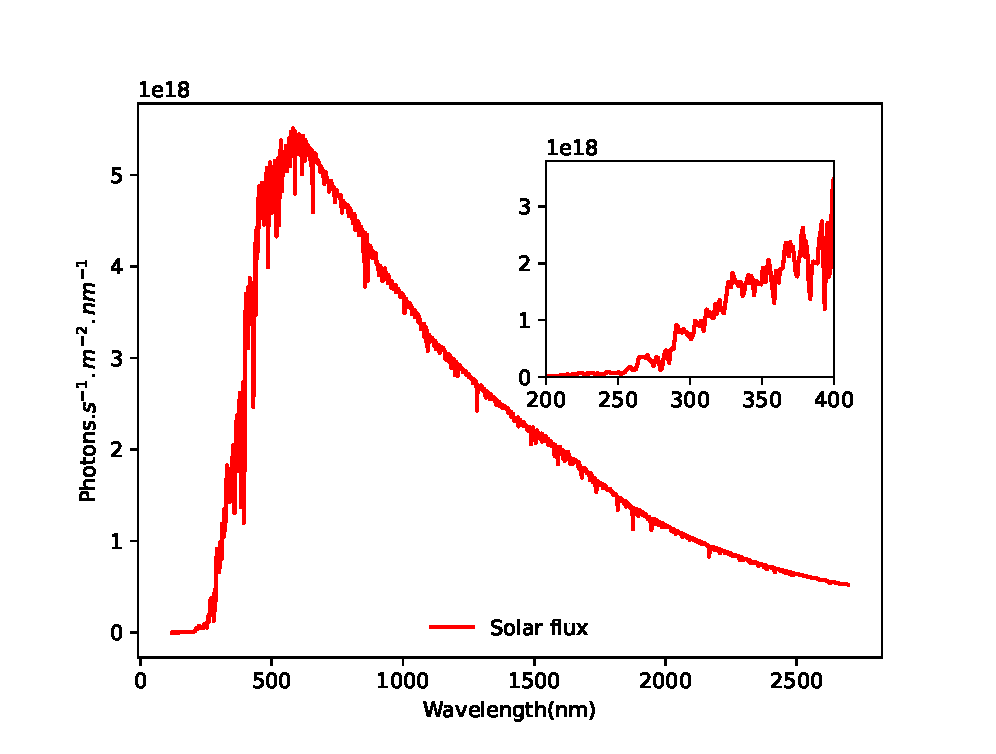
\includegraphics[width=0.7\linewidth]{spectrum_sun.eps}
\end{tabular}
\end{center}
\caption 
{ \label{fig:sun_spec} The Solar spectra from the \href{https://www.stsci.edu/hst/instrumentation/reference-data-for-calibration-and-tools/astronomical-catalogs/calspec}{CALSPEC} database. The Inset plot shows the wavelength range in which \suit is going to observe the Sun, showing the dramatic rise of the spectra in that wavelength band.} 
\end{figure} 
%-----------------------------------------------------------

\suit  payload aims to address the following questions related to the Sun:

\begin{itemize}
    \item Magnetic coupling and dynamics of the solar atmosphere.
    \item Spectral energy distribution in solar flares in NUV
    \item Measure and monitor the spatially resolved solar spectral irradiance in NUV
\end{itemize}

To address these science questions, the necessity of photometric and spectral characterisation is multifold.  \suit, with its capabilities, will be imaging the Sun and the dynamic process such as solar flare and jets etc., occurring in the solar atmosphere (eruptions of different scale) along with magnetic features such as active regions, plage and network regions. Photometric accuracy is key for commenting about the various physical process happening across various scales. The Earth's atmosphere absorbs UV and X-ray emission. Most of the UV radiation below 310 nm is absorbed by Earth's atmosphere, whereas UV radiation beyond 310~nm can penetrate Earth's atmosphere. The main source of absorption below 200~nm is $O_{2}$, while beyond 240 nm it is $O_{3}$. In the 200{--}240~nm region both $O_{2}$ and $O_{3}$ actively take part in the absorption mechanism \cite{haigh07}. So, the Solar spectral irradiance in 200{--}400~nm is one of the key inputs to understand the dynamics and Chemistry of Earth's atmosphere, especially the Ozone-Oxygen cycle, which can be used directly as a key input in modelling the Earth's atmosphere and inferring the Sun-Earth atmosphere connection. With an absolute stellar calibration \suit would provide us the irradiance of the Sun in these bands before it is attenuated by Earth's atmosphere. Accurate spectral characterisation across these bands is key in commenting about the photo chemistry of the upper atmosphere.

To achieve these scientific goals, photometric and spectral calibration of the payload is of utmost importance. An elaborate setup is developed for the calibration of the payload. The payload is kept in a vacuum chamber and maintained at high vacuum ($<10^{-6}$mbar) while the light of desired power and wavelength band from a monochromator is collimated and fed into the vacuum chamber and thereafter, the payload. The collimator used is a flight spare of the \suit payload with similar optical quality as the payload itself. The performed tests help calibrate the photometric counts with the input spectral flux and give a clear idea of the payload spectral response as a whole at its 11 spectral bandpasses. The measured responses are also comparable with simulated payload responses with $\sim 85\%$ similarity.

%%%%%%%%%%%%%%%%%%%%%%%%%%%%%%%%%%%%%%%%%%%%%%%%
\section{Experimental Setup}\label{sec:setup}
%%%%%%%%%%%%%%%%%%%%%%%%%%%%%%%%%%%%%%%%%%%%%%%%

The photometric test and calibration called for an elaborate setup which requires the input of a measured amount of light into the payload within a known band of wavelength. This called for a monochromator to generate monochromatic light within a certain band of wavelength, a collimator to feed the monochromatic light into the payload and a vacuum chamber to operate the payload by simulating space-like conditions.

%%%%%%%%%%%%%%%%%%%%%%%%%%%
\begin{figure*}[ht]
\begin{center}
\begin{tabular}{c}
\includegraphics[trim={2.5cm 0 1.5cm 1.5cm},clip,width=0.8\linewidth]{experimental_setup}
\end{tabular}
\end{center}
\caption 
{ \label{fig:experimentalsetup} Experimental Setup for photometric and spectral calibration of the SUIT payload.} 
\end{figure*}
%%%%%%%%%%%%%%%%%%%%%%%%%%%

\subsection{Contamination control and payload preparation}

\suit is designed to operate in the NUV band of light, making the payload throughput susceptible to particulate and molecular contamination due to high scattering at short wavelengths. Therefore, the payload is assembled and stored in a Class 100 environment with constant purging of level 5 purity (0.0001\% impurity) gaseous nitrogen.
 
 The SUIT CCD has to be maintained at -55\degree C for reliable operation. In space, this is achieved with a radiator plate and a cold finger, which passively cools the CCD by radiating the heat in a direction away from the Sun. Cooling the CCD to that extent in the atmosphere shall cause condensation of water vapor and other contaminants on the CCD surface which is detrimental for CCD electronics and optical throughput. Therefore, the CCD is cooled in a 0.7 m custom-made vacuum chamber at a pressure of $10^{-6}$ mbar to prevent condensation on the CCD.
 Inside the chamber, a jacket is mounted over the cold finger instead of the radiator plate, and cooling is achieved by closed-loop micro-dosing of liquid nitrogen through the jacket.

The vacuum chamber is thoroughly wiped with isopropyl alcohol and is baked at  $70^\circ C$ for 24 hours to remove any contaminants that may exist inside the chamber. Upon reaching room temperature, the level of contamination in the vacuum chamber is verified with a Temperature Controlled Quartz Crystal Microbalance (TQCM). The crystal is kept at a temperature of -10\degree C in high vacuum, making it the coldest surface inside the chamber. Contaminants, if any, get condensed on the TQCM, thus changing the crystal's resonant frequency. The rate of change of frequency measures the amount of contaminant in the chamber. For SUIT, a TQCM count of $\leq 3 Hz/hr$ over 24 hours was considered satisfactory. However, $\leq 2 Hz/hr$ was achieved in practice. \js{Citation Needed}

The photometric and spectral calibration of \suit was performed after payload vibration, acoustic and thermovacuum qualification tests. This required the payload to be transported to various clean rooms and labs. Contamination control protocols were strictly followed during transportation and the tests. However, the payload was subjected to a bakeout at $40 ^\circ C$ for 36 hours before cooling the CCD to avert any risk of contaminating the CCD upon cooling. Post baking, the payload was cooled to room temperature and TQCM verification was performed. The TQCM count was seen to be $< 3 Hz/hr$ after 24 hours of verification, following which the CCD was cooled and the experiments were performed.
 
\subsection{SUIT Collimator}		
The Sun is a collimated light source of finite angular size. Therefore, collimated light must be fed into \suit for testing and calibration. Also, the light should lie in the UV band, and the wavefront error should at least be as good as the payload itself, to ensure good image quality and reliable photometry. For these reasons, the \suit flight spare passes as a viable choice for being a Collimator. The \suit Collimator functions in the opposite sense as that of the payload. Instead of collimated light entering through the front aperture, an illuminated target is kept at the  detector plane of the collimator. This collimated beam of light is then fed into \suit, which eventually gets focused onto the \suit CCD.
	
The optical quality of a system is determined by its wavefront error. A perfect wavefront is a plane in nature. However, optical aberrations introduce undulations in the resultant wavefront, giving rise to peaks and valleys. Therefore, the optical performance of a system is quantified by the RMS deviation of the wavefront about a mean level. Lesser the RMS wavefront error, better is the optical performance of the optical system. The \suit collimator exhibits an RMS wavefront error of 41.4 nm ($\sim \lambda/7 ~ for ~ 300~ nm$) as compared to the \suit payload's 34 nm ($\sim \lambda/9 ~ for ~ 300~ nm$). The zernike coefficients of the collimator are tabulated in Table \ref{table: zernikes}.

The collimator is mounted on an optical table such that the front aperture is aligned with the viewport of the vacuum chamber housing the SUIT payload. The optical bench is designed to rest on six pods bolted to the optical table. A feeler gauge is used to measure any non-planarity between the bench and the pods. Any gaps above 25 microns are filled with shims of appropriate thicknesses. All the bolts fastening the bench and the pods are uniformly torqued to 400 Ncm. 

A small flat mirror is attached to the rear surface of the Collimator primary mirror. A theodolite is used to auto-collimate to the back of the primary mirror, and a larger mirror is placed ahead of the collimator aperture. This mirror is tilted to achieve autocollimation with the previously aligned theodolite, making it in line with the Collimator primary mirror.

An f/25 transmission sphere is used to focus light at the focal plane of the Collimator. The interferometer is tilted by 2.64 degrees with respect to the reference mirror axis, to align it with the secondary mirror arm of the Collimator. The tilt of the interferometer is verified with an autocollimator, and the beam is fed along the chief ray. The light emerges collimated from the front aperture and is retro-reflected back by the large reference mirror into the collimator. The interferogram is recorded, and the RMS wavefront error is used as a reference to determine if any unwanted stress has passed on to the payload bench. The telescope and collimator are of RC design, which causes the wavefront error to change grossly in case of stress induced misalignment.

%%%%%%%%%%%%%%%%%%%%%%%%%%%%%%%%%%%%%%%%%
\begin{table*}[ht]
\caption{Aberrations derived from Zernike coefficients after alignment of SUIT FM and QM.}
\label{table: zernikes}
    \begin{center}
			\begin{tabular}{|c|c|c|}
				\hline
				\rule[-1ex]{0pt}{2.5ex} \textbf{Aberration} & \textbf{\textit{SUIT} payload (nm)} & \textbf{Collimator (nm)}\\
				\hline
				\hline
				\rule[-1ex]{0pt}{2.5ex} \textbf{RMS} & 34 & 41.4 \\
				\hline
				\rule[-1ex]{0pt}{2.5ex} \textbf{PVr} & 196.4 & 210.3 \\
				\hline
				\rule[-1ex]{0pt}{2.5ex} \textbf{Power} & 25 & -4.4 \\
				\hline
				\rule[-1ex]{0pt}{2.5ex} \textbf{Astig X} & -32.7 & 36.7 \\
				\hline
				\rule[-1ex]{0pt}{2.5ex} \textbf{Astig Y} & 22.8 & 0.88 \\
				\hline
				\rule[-1ex]{0pt}{2.5ex} \textbf{Coma X} & -30.8 & -63.3 \\
				\hline
				\rule[-1ex]{0pt}{2.5ex} \textbf{Coma Y} & -9.9 & 28.8 \\
				\hline
				\rule[-1ex]{0pt}{2.5ex} \textbf{Primary Spherical} & -19.8 & -18.8 \\
				\hline
				\rule[-1ex]{0pt}{2.5ex} \textbf{Trefoil X} & -13.9 & -40.4 \\
				\hline
				\rule[-1ex]{0pt}{2.5ex} \textbf{Trefoil Y }& -17.3 & -19.3 \\
				\hline
			\end{tabular}
		\end{center}
	\end{table*} 
%%%%%%%%%%%%%%%%%%%%%%%%%%%%%%%%%%%%%%%%%
	
\subsection{Co-alignment of optical bench and collimator}
Light from the collimator is fed into the vacuum chamber, which is focussed and imaged by \suit. To avoid any loss of light, it is necessary to align the lateral position and tilt of the payload and the collimator. Laterally, the optical axes of both the benches are aligned with millimeter precision, while the tilts are matched with arcmin precision. This intricate alignment of the collimator and the payload is achieved with a theodolite cum autocollimator.

The theodolite is autocollimated with the reference mirror used with the collimator. Using a repeater mirror, the axis is preserved while the theodolite is shifted laterally. Now, a both sided mirror is sighted with the theodolite and its tilt is adjusted to align it with the theodolite axis.
	
The theodolite is shifted to the opposite side of the setup, such that it faces the back of the \suit payload. It is autocollimated with the double sided mirror which aligns the theodolite with the collimator axis. Maintaining autocollimation with a repeater mirror, the theodolite is laterally shifted such that it lines up with the payload alignment cube.
The alignment cube is a highly reflective cube of side 5 mm, mounted outside \suit cover panels. The front and back surfaces of the cube are aligned with respect to the \suit optical axis with a measured amount of offset. The cube is necessary to align the paylaod with the satellite axis, as well as for co-alignment with other payloads or the \suit collimator.
Keeping the theodolite axis invariant, it is laterally shifted to get the alignment cube in its line of sight. The alignment cube offset with respect to the \suit optical axis is set in the theodolite and the payload is shifted within the play of the bolts to achieve autocollimation with the alignment cube. This aligns the payload in the vacuum chamber with the collimator facing it outside the vacuum chamber.
	
An interferometer is used with a f/3.5 transmission sphere to overfill the mirrors of SUIT. The interferometer beam is fed along the optical axis of the payload, which is retroreflected back from the collimator reference mirror. The return beam passes through the collimator optics and reaches the interferometer, which gives the  interferogram. Repeated interferograms are taken, and the fringes are constantly monitored. The interferometer is moved along the z-axis till the fringes appear straight instead of circular, indicating nullification of the power. The point of convergence of the beam from the interferometer is the focal point of the collimator. Light from any target kept at that location emerges collimated. 

\subsection{Monochromator configuration and calibration}
For the photometric and spectral calibration, it is necessary to feed collimated light of a known wavelength band and intensity in \suit.
An Andor Shamrock 500i spectroscope/ monochromator is used with an optical fiber to feed light at the focal plane of the \suit collimator. The optical fiber bundle is linear in nature, with 19 fibers of 0.2 mm thickness arranged in a linear array \js{Model number of optical fiber}. This behaves like an exit slit with a thickness of 0.2 mm.

A Hg2 (Mercury) lamp is used for wavelength calibration of the monochromator and fiber setup. The lamp is kept at the entrance aperture and the central wavelength of a relatively isolated spectral line is set on the monochromator. The fiber face is attached to a photodiode to measure the intensity of the exiting light. Using a micrometer actuator the monochromator exit slit is moved horizontally. The brightness is seen to increase and then starts decreasing, indicating the position of central wavelength of the spectral line. At this position, the fiber is moved vertically to ensure the light arrives at most fibers of the bundle. The brightness is again seen to increase and then decrease, indicating the point of maximum brightness to be the optimized position of the fiber slit. This calibrates the fiber to pick up the same wavelength of light as is chosen in the monochromator software. Now, the monochromator is set to another fairly isolated line within the 200-400 nm band and it is noticed that the intensity of light exiting the fiber is maximum at the set position of the slit. The monochromator and fiber setup is now calibrated to deliver the required wavelength set in the monochromator. The mercury lamp is replaced with a xenon arc lamp which is focussed at the input slit of the monochromator.
 
\section{Photometric Calibration}
Photometric calibration is performed to understand the instrument response to a standard flux of incoming light. This is necessary to quantify the flux of a solar feature from the counts recorded on the SUIT CCD. In this test, an optical fiber is used to feed light from a monochromator at the focal plane of the SUIT collimator. The monochromator uses a 1200 lpmm grating with a nominal dispersion of 1.44 nm/mm. The spectral resolution of the monochromator depends on the entrance slit or the exit slit, whichever is geometrically bigger. In our case, an entrance slit width of 3 mm is used to maximize the light output from the spectrograph. Thus, the emergent monochromatic light has a wavelength band of $3\times 1.44 = 4.32 nm$. The wavelength band is chosen to accommodate the complete transmission spectrum of the narrowband science filter being tested. Light from the exit slit of the spectrograph is carried by an optical fiber. The collecting area of the fiber is slit-like, with a thickness of 200 microns. The fiber terminates as a circular bundle, which is kept at the focal plane of the SUIT collimator and acts as the target for SUIT.
	
	A NIST calibrated photodiode is kept at the exit aperture of the collimator. The wavelengths of the spectrograph and photodiode are set based on the science filter being tested. It is seen that the Xenon lamp spectrum does not change rapidly within 4.32 nm and can be assumed to be flat. Therefore, the output flux measured with the photodiode (in $Wm^{-2}$) can be divided by the wavelength band from the spectrograph to get the spectral flux from the collimator (in $W m^{-2} nm$). Also, the incoming wavelength band is wide enough to accommodate the entire transmission spectrum of the narrowband science filters (typically $< 1~nm$ FWHM). Therefore, the wavelength band incident from the monochromator is sufficient to perform the photometric test with the SUIT payload.
		
	In parallel, the SUIT telescope response has been determined based on the solar spectral irradiance and the throughput of each sub-assembly of the telescope. The experimentally determined throughput is compared with this simulated throughput to check the coherence of the experimental and simulated results. This is necessary to decide the exposure times for the SUIT payload in the 11 science bandpasses at various modes of operation.

 The throughput model for various \suit science filter combinations was designed to predict the counts for a given science filter combination with a sun-as-a-star spectra. The measured wavelength responses of the components are used to estimate the counts. If the photon flux incident on the entrance aperture is given by $P(\lambda)$, then the photoelectron count read at the detector would be given by,

 %%%%%%%%%
 \begin{equation}\label{eq1}
     DN~=~\int~P(\lambda)~R(\lambda)~t~d\lambda
 \end{equation}
 %%%%%%%%%
Where $R(\lambda)$ is the effective area for the specific filter combination and ‘t’ is the exposure time. The effective area $R(\lambda)$ is calculated by multiplying the measured instrumental response of all the optical components in the ray path. So, the filter response is given by

%%%%%%%%%
 \begin{align*}
     & R(\lambda)~=~TF(\lambda)\times PM(\lambda)\times SM(\lambda)\times SF_{i}(\lambda)\times SF_{j}(\lambda)\times L(\lambda)\times QE(\lambda)\times A\\
     & TF(\lambda)\implies~Measured~thermal~filter~wavelength~response \\
     & PM(\lambda)\implies~Measured~primary~mirror~wavelength~response \\
     & SM(\lambda)\implies~Measured~secondary~mirror~wavelength~response \\
     & SF_{i}(\lambda)\implies~Measured~science~filter~response~for~the~i^{th}~filter~on~filter~wheel~1 \\
     & SF_{j}(\lambda)\implies~Measured~science~filter~response~for~the~j^{th}~filter~on~filter~wheel~2  \\
     & L(\lambda)\implies~Measured~field~corrector~lens~wavelength~response \\
     & QE(\lambda)\implies~Measured~quantum~efficiency~of~the~CCD \\
     & A\implies~Area~of~the~entrance~apperture
 \end{align*}
 %%%%%%%%%
 We carry out the comparison between the measurements and the throughput model with the following few steps:

 %%%%%%%%%%
 \begin{itemize}
     \item For a given filter combination we have an image recorded of the optical fiber bundle at the band central wavelength, with the measurement setup shown in figure \ref{fig:experimentalsetup}. From the background corrected optical fiber images we calculate the 99\% encircled energy radius and the total enclosed data counts ($DN_{0.99}$).
     \item The background is estimated by taking the median of dark image (optical fibers closed) pixels.
     \item The photodiode gives the measurement of corresponding input flux($E_{0.99}$) in units of $nW.m^{-2}$ for an input spectral bin of 4.32 nm. The flux is divided by the spectral bin size to get the spectral irradiance per unit area in units of $nW.m^{-2}.nm^{-1}$. The ratio of $DN_{0.99}$ and ${E_{0.99}}$ tells us about the expected counts for any given input flux, $F~=~\frac{DN_{0.99}}{E_{0.99}}$ in units of $ADC~counts.s^{-1}/(nW.m^{-2}.nm^{-1})$.
     \item We use a composite SOLar STelar Irradiance Comparison Experiment (SOLSTICE; 115 - 320 nm) onboard the SOlar Radiation and Climate Experiment (SORCE) \cite{rottman05,harder05,mcclintock05} satellite and SOLar SPECtrometer (SOLSPEC) \cite{thuillier09} solar spectrum as our standard for solar radiation. Using the spectra we can calculate the total energy input from Sun for the concerned filter within the wavelength extent, $E_{\odot}~=~\int_{\lambda_{}}^{\lambda_{2}}~P(\lambda)~d\lambda$, where $P(\lambda)$ is the Solstice, Solspec composite solar spectra. Here, $\lambda_{1}-\lambda_{2}$ is the extent of the concerned band.
     \item Using eqn.\ref{eq1} along with the aforementioned spectra, we can calculate the expected count observed (i.e. $DN_{throughput}~=~\int~P(\lambda)~R(\lambda)~t~d\lambda$) for a given filter combination.
     \item The ratio inferred from the measurement of the input energy measured by the photdiode, and the total counts within 99\% encircled energy radius as described for the specific filter combination, F (in units of $ADC~counts.s^{-1}/(nW.m^{-2}.nm^{-1})$) can be used to calculate the expected counts from the Sun given by $DN_{measured}~=~E_{\odot}\times~F$
     \item In table~\ref{tab:throughput} we list out the comparison between the solar counts inferred from our measurements and the counts calculated from the throughput model, for some of the filter combinations. The values are in agreement within 15\%.
 \end{itemize}
 %%%%%%%%%%

 %-----------------------------------------------------------
\begin{table*}[ht]
\caption{Comparison of the throughut model with the counts inferred from the measurements.} 
\label{tab:throughput}
\begin{center}
\begin{tabular}{|||c|c|c|c|||}
\hline
Science & Photoelectron counts calculated & Photoelectron counts calculated & Ratio of \\
filter & from measurement & from throughput model &  \\
 & $DN_{measured}~=~E_{\odot}\times~F$ & $DN_{throughput}~=~\int~P(\lambda)~R(\lambda)~t~d\lambda$ & $\frac{DN_{measured}}{DN_{throughput}}$\\
 & (photo electrons/s) & (photo electrons/s) & \\
\hline
NB2 & 53142 & 49099 & 1.08 \\
NB3 & 18531 & 15520 & 1.19 \\
NB4 & 35040 & 36717 & 0.95 \\
NB5 & 124116 & 131625 & 0.943 \\
NB6 & 105138 & 107064 & 0.98 \\
NB8 & 26523 & 24096 & 1.1 \\
BB3 & 511722 & 434532 & 1.18 \\
\hline

\end{tabular}
\end{center}
\end{table*}
%-----------------------------------------------------------

%################################### 
\section{Spectral Calibration}
%###################################
	
The purpose of Spectral calibration is to verify the wavelength transmission profile of the SUIT payload with various science filters. For spectral calibration, a holographic grating of 2400 lpmm was used, blazed at 220 nm wavelength. The nominal dispersion of this grating is 0.74 nm/mm. The entrance slit width is set at 200 microns. Therefore, the wavelength bin being fed into SUIT is $(0.74 nm/mm \times 0.2 mm= 0.148 nm)$ nm. Readings are taken across the transmission spectrum of the science filter without any spectral overlap to keep adjacent readings independent of each other. The total energy is counted at each measured wavelength, and the spectral response of the entire telescope for all filters is measured.
	
Following this, the entrance slit width of the monochromator is increased to 3 mm, and the light output is measured from the clear aperture of the collimator with a NIST photodiode to verify the spectral flux being fed into the SUIT payload. This information can be used to get a radiometric calibration to the measured spectral flux. The spectral calibration is calculated from the measurements from the following steps:

 %%%%%%%%%%
 \begin{itemize}
 \item With the instrument setup described the input from the optical fiber bundle is imaged for various filter combinations. From the background corrected fiber images we calculate the 99\% encircled energy radius.
 \item The background is estimated by taking the median of dark image (optical fibers closed) pixels.
 \item The total counts within the 99\% encircled energy radius is calculated, $C_{i}$ in units of ADC counts/s.
 \item The corresponding energy input from photo-diode measurement is $E_{i}$ in units of $nW.m^{-2}.nm^{-1}$.
 \item The same measurement can be carried out for various wavelength points within the wavelength range of the concerned filter combination. The ratio of these two quantities, $F_{i}~=~\frac{C_{i}}{E_{i}}$ 
the spectral calibration for that filter combination in units of $ADC~counts.s^{-1}/(nW.m^{-2}.nm^{-1})$ as a function of wavelength.
 \end{itemize}
 %%%%%%%%%%

In figure \ref{fig:nb2_images} we show the captured images for the NB2 filter combination at various wavelengths. The measurement wavelength and the calculated 99\% encircled energy radius is quoted at the top of each panel.  In fig.~\ref{fig:sepc_calib} we plot the spectral calibration of various filter combinations. The x and y error bars in fig.~\ref{fig:sepc_calib} are the wavelength bins for the given input slit size, and the Poisson uncertainty of the measured ADC counts respectively.

%%%%%%%%%%%%%%%%%%%%%%%%%%%
\begin{figure*}[ht]
\begin{center}
\begin{tabular}{c}
\includegraphics[width=0.8\linewidth]{nb2_images.pdf}
\end{tabular}
\end{center}
\caption 
{ \label{fig:nb2_images} Images captured at various wavelengths for the NB2 filter combination. The measurement wavelength and the 99\% encircled energy radius is quoted at the top of each panel. The axis of the images are in pixels. The pixels are 12 $\mu$m in dimension.} 
\end{figure*}
%%%%%%%%%%%%%%%%%%%%%%%%%%%

%%%%%%%%%%%%%%%%%%%%%%%%%%%
\begin{figure*}[ht]
\begin{center}
\begin{tabular}{c}
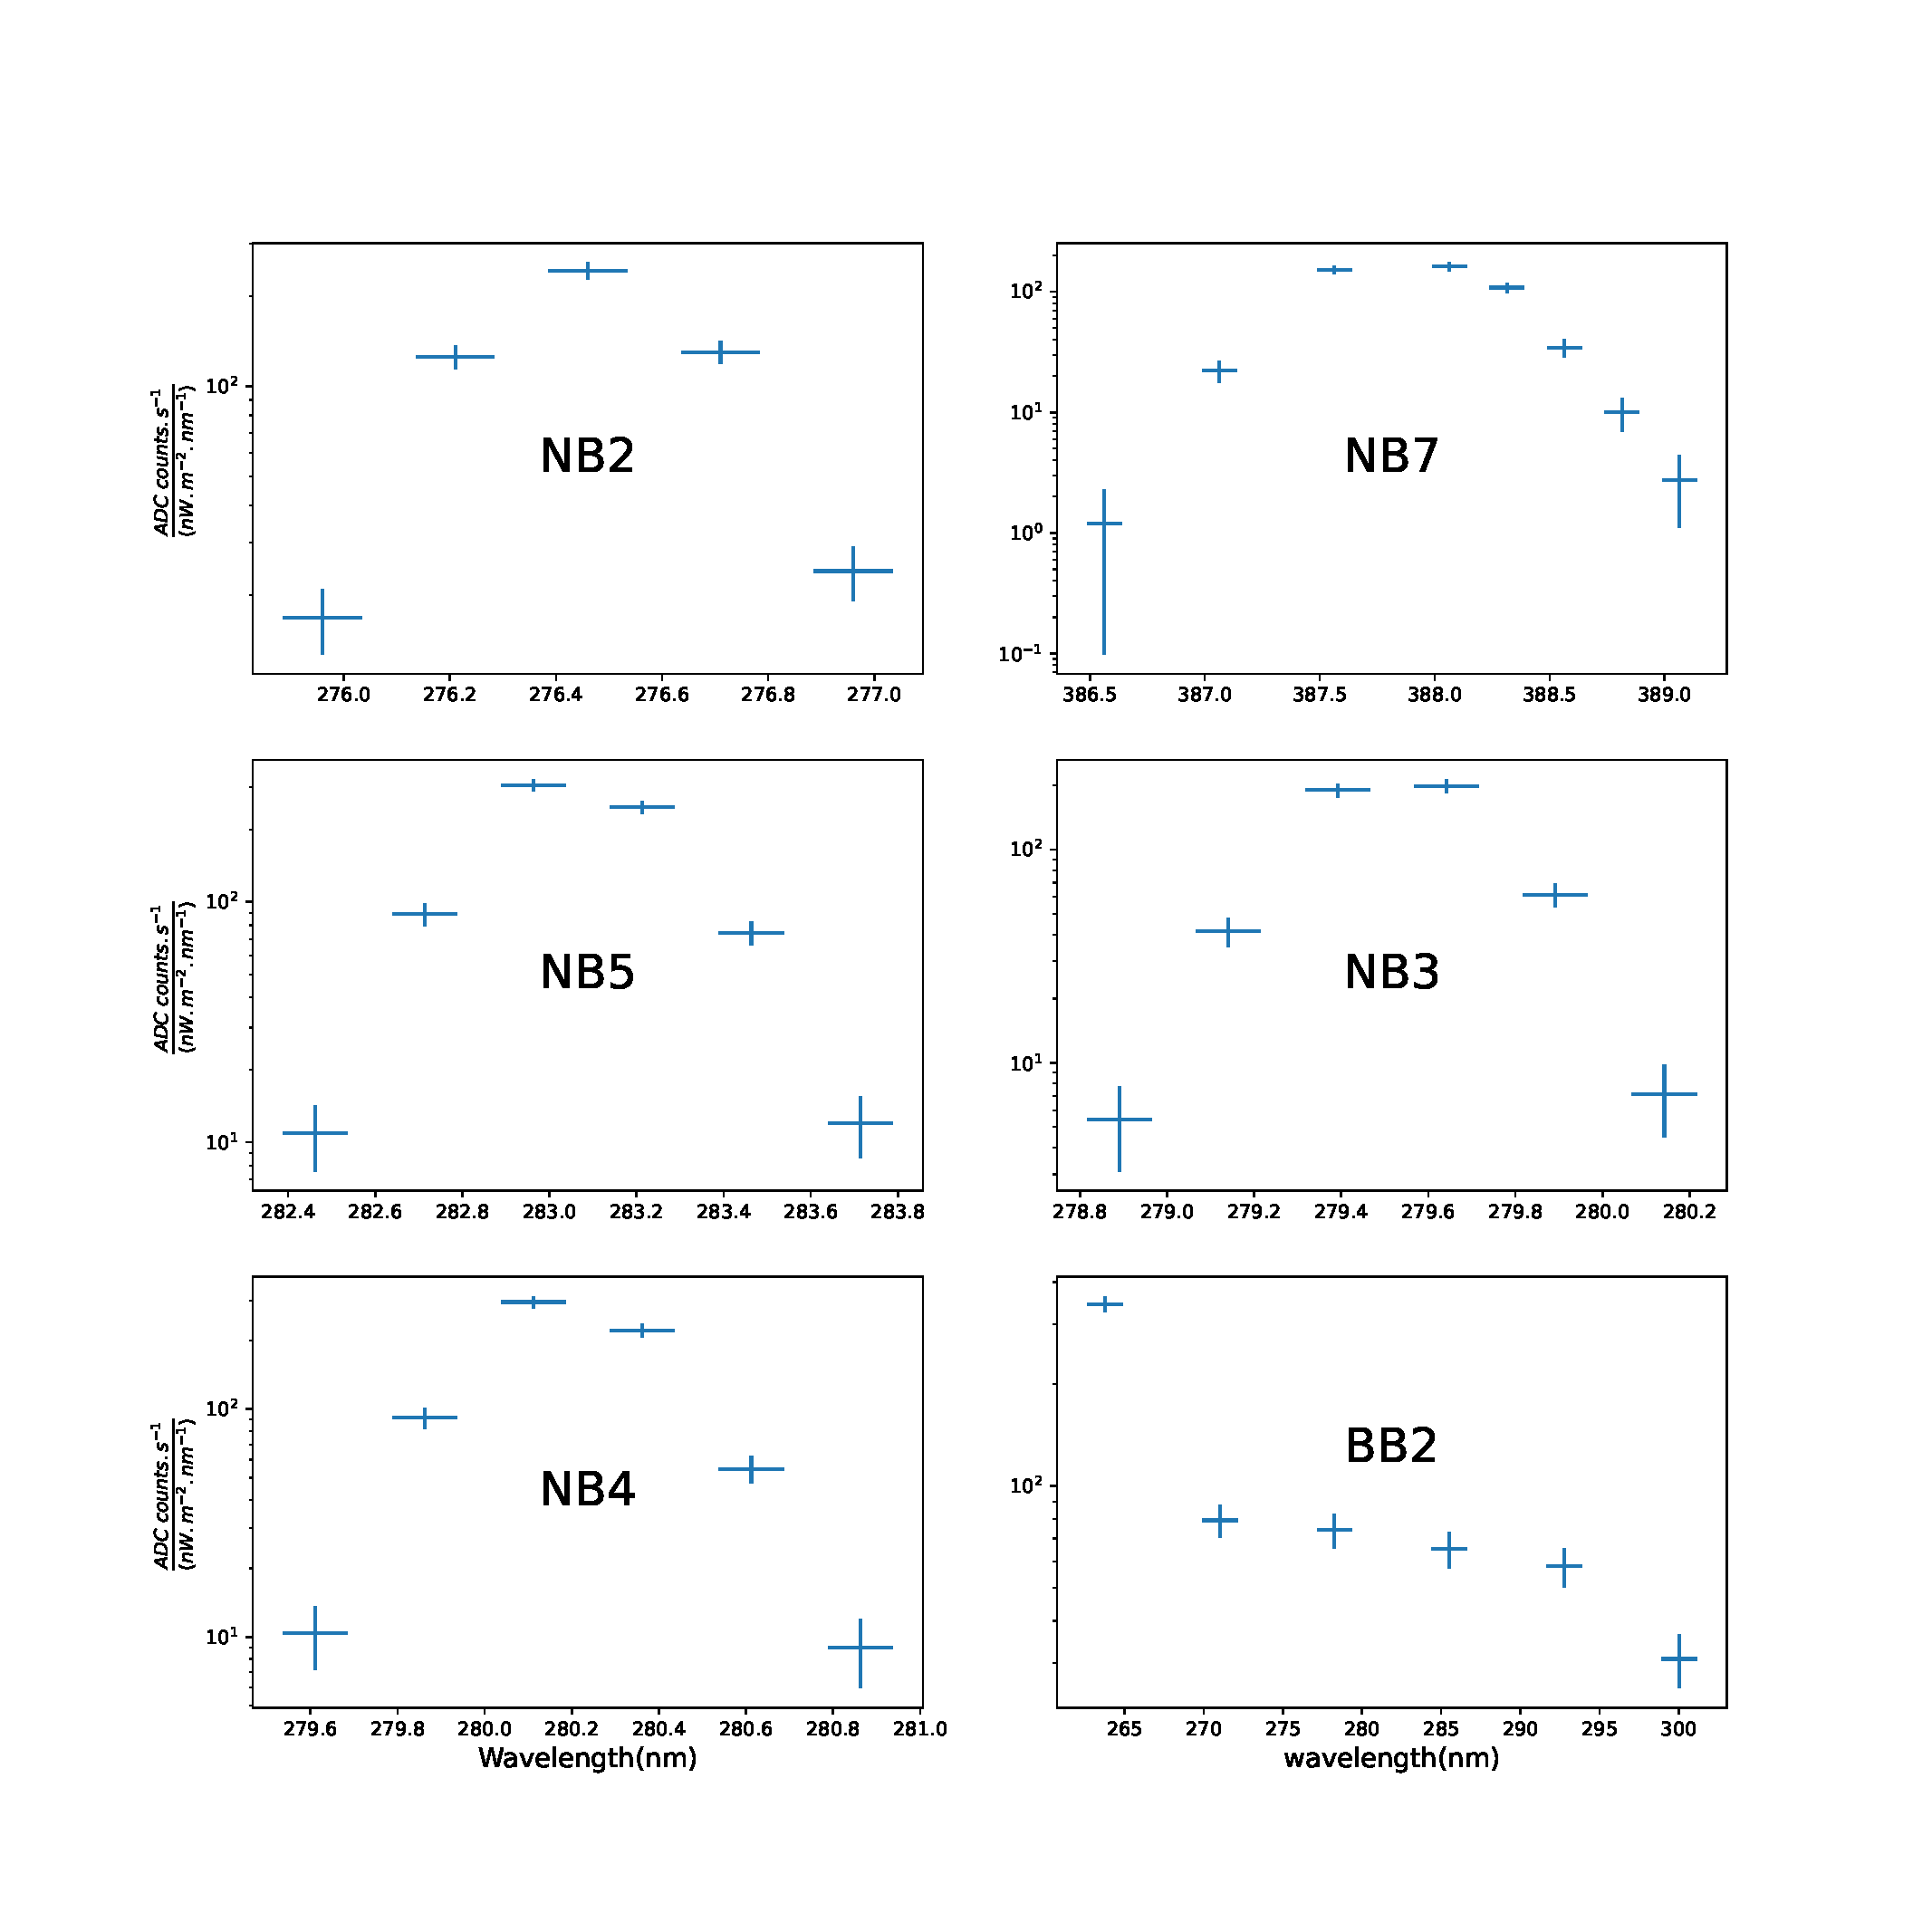
\includegraphics[trim={2.5cm 2.5cm 3cm 4cm},clip,width=0.8\linewidth]{spec_calib.eps}
\end{tabular}
\end{center}
\caption 
{ \label{fig:sepc_calib} Spectral calibration for various filter combinations inferred from the imaging measurements. The x errors are given by the wavelength bins for the given input slit size. The y errors are given by the Poisson uncertainty of the measured ADC counts.} 
\end{figure*}
%%%%%%%%%%%%%%%%%%%%%%%%%%%

%###################################
\section{Discussion \& Conclusion}\label{sec:conc}
%###################################

The photometric calibration and full payload spectral verification for the \suit are presented in this paper. The experimental setup consists of the payload maintained in a high vacuum environment and a collimator feeding light from a monochromator. The collimator had to have a high reflectance in UV with comparable optical quality to the payload. Therefore, the flight spare model of \suit is used to meet this purpose.

Photometric calibration is essential to correlate the counts gathered on \suit CCD for a specific filter combination to the incoming solar radiation. The intensity of collimated light within a certain wavelength band is measured with a NIST calibrated photodiode and fed into the payload. The measured response of the payload is seen to agree with simulated values within a margin of 15\%. 

However, the bandpasses NB1, BB1 and BB2 are below 250 nm and, therefore, get attenuated in the atmosphere. Moreover, the Xenon light source transmission is very low \sr{Maybe we should mention how low?} in these wavelengths. Thus, the data gathered has low SNR and is unreliable for performing photometry. On the other hand, the exposure time for the NB7 filter is very low \sr{Maybe we should put the table for nominal exposure time with the science filters table?} as it operates at 388 nm, which is close to UV transmission. Therefore, the photometry is unreliable for this filter due to measurement errors.

For the spectral characterization, the wavelength bin of the input light is reduced, and the response is measured across the transmission bandpass of the science filters. It is seen that the spectral response of the instrument matches the central wavelengths \suit is designed to observe.

%###################################

%xxxxxxxxxxxxxxxxxxxxxxxxxxxxxxxxxxxxxxxxxxxxxxxxxxxxxxxxxxxxxxxxxxxxxxxxxxxxxxxxxxxxxxxxxxxxxxxxx

% \disclosures 
\subsection*{Disclosures}
%Conflicts of interest should be declared under a "Disclosures" header. If the authors have no relevant financial interests in the manuscript and no other potential conflicts of interest to disclose, a statement to this effect should also be included in the manuscript.


\subsection* {Code, Data, and Materials Availability} 
%In support of open scientific exchange, SPIE journals require Code, Data, and Materials Availability Statements in all accepted papers. This requirement went into effect on 1 May 2023. These statements should describe how to access any data that would be required to replicate or interpret the findings reported in the paper. Authors are encouraged to make the data and code related to the manuscript publicly available whenever possible, and utilize repositories that are well-known to the field (FigShare, Github, CodeOcean, etc.). If the data or code cannot be made publicly available, the authors should state the reason and explain how it can be obtained. Likewise, if data sharing is not applicable, the statement must say so. Example statements may be found in the Author Guidelines for the journal.


\subsection* {Acknowledgments}
%This unnumbered section is used to identify those who have aided the authors in understanding or accomplishing the work presented and to acknowledge sources of funding. 


%%%%% References %%%%%

\bibliography{report}   % bibliography data in report.bib
\bibliographystyle{spiejour}   % makes bibtex use spiejour.bst

%%%%% Biographies of authors %%%%%

\vspace{2ex}\noindent\textbf{First Author} is an assistant professor at the University of Optical Engineering. He received his BS and MS degrees in physics from the University of Optics in 1985 and 1987, respectively, and his PhD degree in optics from the Institute of Technology in 1991.  He is the author of more than 50 journal papers and has written three book chapters. His current research interests include optical interconnects, holography, and optoelectronic systems. He is a member of SPIE.

\vspace{1ex}
\noindent Biographies and photographs of the other authors are not available.

\listoffigures
\listoftables

%\end{spacing}
\end{document}














\section{Introduction}
\label{sect:intro}  % \label{} allows reference to this section
This document shows the format and appearance of a manuscript prepared for submission to SPIE journals. Note that this template is only intended to be used as a guideline for author convenience. It is designed for optimum clarity and ease of reading for editors and reviewers, but the template does not reflect the final page layout of a published journal paper. Accepted papers are professionally typeset in XML according to the layout and design of the journal. 

\subsection{Use of This Document}

This document is prepared using LaTeX2e\cite{Lamport94,Goossens97} with the class file {\ttfamily spieman.cls}.  The LaTeX source file used to create this document is {\ttfamily article.tex}, which contains important formatting information embedded in it. Authors may use it as a template to create their own manuscript. While LaTeX properly handles most formatting issues, the author may occasionally need to intervene to obtain a satisfactorily  formatted manuscript.

\subsection{English}

Authors are strongly encouraged to follow the principles of sound technical writing, as found in Refs.~\citenum{Alred03} and \citenum{Perelman97}, for example. In addition, good English usage is essential. Authors whose native language is not English may wish to collaborate with a colleague whose English skills are more advanced. Alternatively, you may wish to have your manuscript professionally edited prior to submission by Editage, our recommended independent editorial service: \linkable{https://www.editage.com/spie/}. SPIE authors will receive a 15\% discount off their services. A spell checker can be helpful to discover misspelled words, but authors should also proofread their papers carefully prior to submission. Manuscripts that do not meet acceptable English standards or lack clarity may be rejected.

\subsection{Page Setup and Fonts}

All text and figures, including footnotes, must fit inside a text area 6.5 in.\ wide by 9 in.\ high (16.51 by 22.86 cm). Manuscripts must be formatted for US letter paper, on which the margins should be 1 in.\ (2.54 cm) on the top, 1 in.\ on the bottom, and 1 in.\ on the left and right. 

The Times New Roman font is used throughout the manuscript, in the sizes and styles shown in Table~\ref{tab:fonts}. If this font is not available, use a similar serif font. The manuscript should not contain headers or footers. Pages should be numbered.

\begin{table}[ht]
\caption{Fonts sizes and styles.} 
\label{tab:fonts}
\begin{center}       
\begin{tabular}{|l|l|} %% this creates two columns
%% |l|l| to left justify each column entry
%% |c|c| to center each column entry
%% use of \rule[]{}{} below opens up each row
\hline
\rule[-1ex]{0pt}{3.5ex}  Document entity & Brief description  \\
\hline\hline
\rule[-1ex]{0pt}{3.5ex}  Article title & 16 pt., bold, left justified  \\
\hline
\rule[-1ex]{0pt}{3.5ex}  Author names & 12 pt., bold, left justified   \\
\hline
\rule[-1ex]{0pt}{3.5ex}  Author affiliations & 10 pt., left justified   \\
\hline
\rule[-1ex]{0pt}{3.5ex}  Abstract & 10 pt.  \\
\hline
\rule[-1ex]{0pt}{3.5ex}  Keywords & 10 pt.  \\
\hline
\rule[-1ex]{0pt}{3.5ex}  Section heading & 12 pt., bold, left justified  \\
\hline
\rule[-1ex]{0pt}{3.5ex}  Subsection heading & 12 pt., italic, left justified  \\
\hline
\rule[-1ex]{0pt}{3.5ex}  Sub-subsection heading & 11 pt., italic, left justified  \\
\hline
\rule[-1ex]{0pt}{3.5ex}  Normal text & 12 pt. \\
\hline
\rule[-1ex]{0pt}{3.5ex}  Figure and table captions &  10 pt. \\
\hline 
\end{tabular}
\end{center}
\end{table} 

\section{Parts of Manuscript}

This section describes the normal structure of a manuscript and how each part should be handled. The appropriate vertical spacing between various parts of this document is achieved in LaTeX through the proper use of defined constructs, such as \verb|\section{}|. 

\subsection{Title and Author Information}
\label{sect:title}
The article title appears left justified at the top of the first page. The title font is 16 pt., bold. The rules for capitalizing the title are the same as for sentences; only the first word, proper nouns, and acronyms should be capitalized. Do not begin titles with articles (for example, a, an, the) or prepositions (for example, on, by, etc.). The word ``novel'' should not appear in the title, as publication will imply novelty. Avoid the use of acronyms in the title, unless they are widely understood.

The list of authors immediately follows the title, 18 points below. The font is 12 pt., bold and the author names are left justified. The author affiliations and addresses follow the names, in 10-pt., normal font and left justified. For multiple affiliations, each affiliation should appear on a separate line. Superscript letters (a, b, c, etc.) should be used to associate multiple authors with their respective affiliations. The corresponding author should be identified with an asterisk, and that person's email address should be provided below the keywords.

\subsection{Abstract}
The abstract should be a summary of the paper and not an introduction. Because the abstract may be used in abstracting journals, it should be self-contained (i.e., no numerical references) and substantive in nature, presenting concisely the objectives, methodology used, results obtained, and their significance. Please note that the following journals require the use of structured abstracts in manuscript submissions: \textit{Neurophotonics}, the \textit{Journal of Biomedical Optics}, and the \textit{Journal of Medical Imaging}. Structured abstracts are encouraged for the \textit{Journal of Micro/Nanolithography, MEMS, and MOEMS}. Helpful guidelines for structured abstracts are available on the website of the journal.

\subsection{Subject terms/Keywords}
Keywords are required. Please provide 3-6 keywords related to your paper. 

\subsection{Body of Paper}
The body of the paper consists of numbered sections that present the main findings. These sections should be organized to best present the material.

To provide transition elements in your paper, it is important to refer back (or forward) to specific sections. Such references are made by indicating the section number, for example, ``In Sec.\ 2 we showed...'' or ``Section 2.1 contained a description...'' If the word Section, Reference, Equation, or Figure starts a sentence, it is spelled out. When occurring in the middle of a sentence, these words are abbreviated Sec., Ref., Eq., and Fig. 

At the first occurrence of an acronym, spell it out followed by the acronym in parentheses, for example, charge-coupled diode (CCD).

\subsection{Footnotes}
Textual footnotes should be used rarely to present important documentary or explanatory material whose inclusion in the text would be distracting.\footnote{Example of a footnote.} Due to problems with HTML display, use of footnotes should generally be avoided. If absolutely necessary, the footnote mark must come at the end of a sentence. To insert a footnote, use the {\verb|\footnote{}|} command.

\subsection{Appendices}
Brief appendices may be included when necessary, such as derivations of equations, proofs of theorems, and details of algorithms. Equations and figures appearing in appendices should continue sequential numbering from earlier in the paper.

\subsection{Disclosures}
Conflicts of interest should be declared under a separate header. If the authors have no competing interests to declare, then a statement should be included declaring no conflicts of interest. For assistance generating a disclosure statement, see the form available from  the International Committee of Medical Journal Editors website: \linkable{http://www.icmje.org/conflicts-of-interest/} 

\subsection{Code, Data, and Materials Availability}
In support of open scientific exchange, SPIE journals require Data and Code Availability Statements in all accepted papers. This requirement went into effect on 1 May 2023. These statements should describe how to access any data that would be required to replicate or interpret the findings reported in the paper.  

\subsection{Acknowledgments}
Acknowledgments and funding information should be added after the conclusion, and before references. Include grant numbers and the full name of the funding body. The acknowledgments section does not have a section number.

\subsection{References}
The References section lists books, articles, and reports that are cited in the paper. This section does not have a section number. The references are numbered in the order in which they are cited. Examples of the format to be followed are given at the end of this document.

The reference list at the end of this document is created using BibTeX, which looks through the file {\ttfamily report.bib} for the entries cited in the LaTeX source file.  The format of the reference list is determined by the bibliography style file {\ttfamily spiejour.bst}, as specified in the \\ \verb|\bibliographystyle{spiejour}| command.  Alternatively, the references may be directly formatted in the LaTeX source file.

For books\cite{Lamport94,Alred03,Goossens97} the listing includes the list of authors (initials plus last name), book title (in italics), page or chapter numbers, publisher, city, and year of publication.  Journal-article references \cite{Metropolis53,Harris06} include the author list, title of the article (in quotes), journal name (in italics, properly abbreviated), volume number (in bold), inclusive page numbers or citation identifier, and year.  A reference to a proceedings paper or a chapter in an edited book\cite{Gull89a} includes the author list, title of the article (in quotes), conference name (in italics), editors (if appropriate), volume title (in italics), volume number if applicable (in bold), inclusive page numbers, publisher, city, and year.  References to an article in the SPIE Proceedings may include the conference name, as shown in Ref.~\citenum{Hanson93c}.

The references are numbered in the order of their first citation. Citations to the references are made using superscripts, as demonstrated in the preceding paragraph. One may also directly refer to a reference within the text, for example, ``as shown in Ref.~\citenum{Metropolis53} ...''  Two or more references should be separated by a comma with no space between them. Multiple sequential references should be displayed with a dash between the first and last numbers \cite{Alred03,Perelman97,Lamport94,Goossens97,Metropolis53}. 

\subsubsection{Reference linking and DOIs}
A Digital Object Identifier (DOI) is a unique alphanumeric string assigned to a digital object, such as a journal article or a book chapter, that provides a persistent link to its location on the internet. The use of DOIs allows readers to easily access cited articles. Authors should include the DOI at the end of each reference in brackets if a DOI is available. See examples at the end of this manuscript. A free DOI lookup service is available from CrossRef at \\\linkable{http://www.crossref.org/freeTextQuery/}. The inclusion of DOIs will facilitate reference linking and is highly recommended. 

In the present LaTeX template, the author needs to add the DOI reference by including it in a ``note'' in the bibliography file, as shown in the file {\verb+report.bib+}, for example, \\ {\verb+note = "[doi:10.1117/12.154577]"+}. The DOI may be used by the reader to locate that document with the link: {\verb+http://dx.doi.org10.1117/12.154577+}. 

\subsection{Biographies}
A brief professional biography of approximately 75 words may be provided for each author, if available. Biographies should be placed at the end of the paper, after the references. Personal information such as hobbies or birthplace/birthdate should not be included. Author photographs are not published.

\section{Section Formatting}
\label{sect:sections}
In LaTeX, a new section is created with the \verb|\section{}| command, which automatically numbers the sections. Sections will be numbered sequentially, starting with the first section after the abstract, except for the acknowledgments and references. (Note that numbering of section headings is not required, but the numbering must be consistent if used.) All section headings should be left justified.

Main section headings are in 12-pt. bold font, left-justified and in title case, where important words are capitalized.

Paragraphs that immediately follow a section heading are leading paragraphs and should not be indented, according to standard publishing style. The same goes for leading paragraphs of subsections and sub-subsections. Subsequent paragraphs are standard paragraphs, with 0.2-in (5 mm) indentation. There is no additional space between paragraphs. In LaTeX, paragraphs are separated by blank lines in the source file. Indentation of the first line of a paragraph may be avoided by starting it with \verb|\noindent|.

\subsection{Subsection Headings}
All important words in a subsection (level 1) header are capitalized. Subsection numbers consist of the section number, followed by a period, and the subsection number within that section, without a period at the end. The heading is left justified and its font is 12 pt. italic.

\subsubsection{Sub-subsection headings}
The first word of a sub-subsection is capitalized. The rest of the text is not capitalized, except for proper names and acronyms (the latter should only be used if well known). The heading is left justified and its font is 11 pt. italic. 

\section{Figures and Tables}

\subsection{Figures}

Figures are numbered in the order in which they are called out in the text. They should appear in the document in numerical order and as close as possible to their first reference in the text. It may be necessary to move figures or tables around to enhance readability. LaTeX will attempt to place figures at the top or bottom of a page in which they are first referenced.

Figures, along with their captions, should be separated from the main text by  0.2 in.\ or 5 mm and centered. Figure captions are centered below the figure or graph. Figure captions start with the abbreviation ``Fig'' in front of the figure number, followed by a period, and the text in 10-pt. font. See Fig.~\ref{fig:example} for an example.

\begin{figure}
\begin{center}
\begin{tabular}{c}
\includegraphics[height=5.5cm]{mcr3b.eps}
\end{tabular}
\end{center}
\caption 
{ \label{fig:example}
Example of a figure caption. } 
\end{figure} 

Authors may wish to create figures consisting of two or more images, in which case, they should be neatly arranged in a rectangular array.  In no case, should the article's text be wrapped around a figure. Figure~\ref{fig:example2} shows two side-by-side images. When a figure contains more than one image, the author must submit them as a single image file. Further details about figure formatting can be found in the author guidelines for each specific SPIE journal: \\
\linkable {https://www.spiedigitallibrary.org/journals/journal-authors}. 

\begin{figure}
\begin{center}
\begin{tabular}{c}
\includegraphics[height=5.5cm]{fig2.eps}  % fig2 includes two images 
\\
(a) \hspace{5.1cm} (b)
\end{tabular}
\end{center}
\caption 
{ \label{fig:example2}
Example of a figure containing multiple images: (a) sun and (b) blob. Figures containing multiple images must be submitted to SPIE as a single image file.} 
\end{figure} 

\subsection{Tables}
Tables are numbered in the order in which they are referenced. They should appear in the document in numerical order and as close as possible to their first reference in the text. It is preferable to have tables appear at the top or bottom of the page, if possible. Table captions are handled identically to those for figures, except that they appear above the table. See Table~\ref{tab:fonts} for an example.

\subsection{Video}
Acceptable file formats, including MOV (.mov), MPEG (.mpg), and MP4 (.mp4), are playable using standard media players, such as VLC or Windows Media Player. The recommended maximum size for each video file is 10-12 MB. Authors may insert a representative still image from the video file in the manuscript as a figure. The caption label will be linked by the publisher to the actual video file. The video may also be mentioned in an existing figure caption. Multimedia files are treated in the same manner as figures and they will be numbered sequentially with normal figures.  The video number, file type, and file size should be included in parentheses at the end of the figure caption. See Figure \ref{vid:satellite} for an example.

\begin{video}
\begin{center}
{\includegraphics[height=5cm]{satellite.eps}}
\\
\end{center}
\caption{\label{vid:satellite}This satellite is a still image from Video 1 (Video 1, MPEG, 2.5 MB).}
\end{video}

\appendix    % this command starts appendixes

\section{Miscellaneous Formatting Details}
\label{sect:misc}
At times it may be desired, for formatting reasons, to break a line without starting a new paragraph. In a LaTeX source file, a linebreak is created with \verb|\\|.


\subsection{Formatting Equations}
Equations may appear inline with the text, if they are simple, short, and not of major importance; for example, $\beta = b/r$.  Important equations appear on their own line.  Such equations are centered.  For example, ``The expression for the field of view is
\begin{equation}
\label{eq:fov}
2 a = \frac{(b + 1)}{3c} \, ,
\end{equation}
where $a$ is the ...''  Principal equations are numbered, with the equation number placed within parentheses and right justified.  

Equations are considered to be part of a sentence and should be punctuated accordingly. In the above example, a comma appears after the equation because the next line is a subordinate clause. If the equation ends the sentence, a period should follow the equation. The line following an equation should not be indented unless it is meant to start a new paragraph. Indentation after an equation is avoided in LaTeX by not leaving a blank line between the equation and the subsequent text.

References to equations include the equation number in parentheses, for example, ``Equation~(\ref{eq:fov}) shows ...'' or ``Combining Eqs.~(2) and (3), we obtain...'' Note that the word ``Equation'' is spelled out if it begins a sentence, but is abbreviated as ``Eq.'' otherwise. Using a tilde in the LaTeX source file between two characters avoids unwanted line breaks, for example between ``Eq.'' and the following equation number..

\subsection{Formatting Theorems}

To include theorems in a formal way, the theorem identification should appear in a 10-point, bold font, left justified, and followed by a period.  The text of the theorem continues on the same line in normal, 10-pt. font, achieved in LaTeX using \verb|\footnotesize|.  For example, 

\vspace{2ex}\noindent{\footnotesize\textbf{Theorem 1.} For any unbiased estimator...}

